% -=-=-=-=-=-=-=-=-=-=-=-=-=-=-=-=-=-=-=-=-=-=-=-=-=-=-=-=-=-=-=-=-=-=-=-=-=-=-=
% COURS MUI
% Bertrand Hochet  Pierre Favrat  C�dric Bornand
% created February 2014
% version 
% -=-=-=-=-=-=-=-=-=-=-=-=-=-=-=-=-=-=-=-=-=-=-=-=-=-=-=-=-=-=-=-=-=-=-=-=-=-=-=
\documentclass[10pt,a4paper]{book}
\usepackage[latin1]{inputenc}
\usepackage[T1]{fontenc}
\usepackage[english,english,french]{babel}

%\usepackage[utf8]{inputenc}
\usepackage[french]{babel}
% -=-=-=-=-=-=-=-=-=-=-=-=-=-=-=-=-=-=-=-=-=-=-=-=-=-=-=-=-=-=-=-=-=-=-=-=-=-=-=
% 
% 
%
% -=-=-=-=-=-=-=-=-=-=-=-=-=-=-=-=-=-=-=-=-=-=-=-=-=-=-=-=-=-=-=-=-=-=-=-=-=-=-=


% divers packages utiles
\usepackage{graphicx}
\usepackage{ifthen}
\usepackage{amssymb}
\usepackage{chngpage}
\usepackage{lastpage}
\usepackage{listings}
\usepackage{amsmath}
\usepackage{amssymb,amsfonts,textcomp}
\usepackage{color}
\usepackage{colortbl}
\usepackage{xcolor}
\usepackage{amssymb}
%\usepackage{algorithm,algorithmic}
\usepackage{algorithmic}
\usepackage{algorithm}
\usepackage{array}
\usepackage{supertabular}
\usepackage{multirow} 
\usepackage{hhline}
\usepackage{hyperref}
%\usepackage{tikz}
\hypersetup{pdftex, colorlinks=true, linkcolor=blue, citecolor=blue, filecolor=blue, urlcolor=blue, pdftitle=microinformatique, pdfauthor=linuxmint , pdfsubject=Chapitre 01 - Introduction, pdfkeywords=}
\usepackage{fancyhdr}

% taille imprimable
\usepackage{fullpage} % Agrandit les dimensions du texte (hauteur, largeur,
                     % etc.) par rapport  celles par dfaut. Attention
                     % ce package ne se trouve pas dans toutes les
                     % distributions LaTeX

% -=-=-=-=-=-=-=-=-=-=-=-=-=-=-=-=-=-=-=-=-=-=-=-=-=-=-=-=-=-=-=-=-=-=-=-=-=-=-=
\usepackage[a4paper, top=1cm, bottom=2.5cm, left=2cm, headheight=6mm, headsep=5mm, marginparwidth=0.5cm, marginparsep=4mm, heightrounded, includehead]{geometry} 

% -=-=-=-=-=-=-=-=-=-=-=-=-=-=-=-=-=-=-=-=-=-=-=-=-=-=-=-=-=-=-=-=-=-=-=-=-=-=-=
 
%
\newcommand\textstyleInternetlink[1]{\textcolor{blue}{#1}}

\newcommand\textsubscript[1]{\ensuremath{{}_{\text{#1}}}}
\makeatletter
\newcommand\arraybslash{\let\\\@arraycr}
\makeatother
% Footnote rule
\setlength{\skip\footins}{0.119cm}
\renewcommand\footnoterule{\vspace*{-0.018cm}\setlength\leftskip{0pt}\setlength\rightskip{0pt plus 1fil}\noindent\textcolor{black}{\rule{0.25\columnwidth}{0.018cm}}\vspace*{0.101cm}}
% Pages styles
\makeatletter
\newcommand\ps@Standard{
  \renewcommand\@oddhead{}
  \renewcommand\@evenhead{\@oddhead}
  \renewcommand\@oddfoot{}
  \renewcommand\@evenfoot{}
  \renewcommand\thepage{\arabic{page}}
}
\makeatother
\pagestyle{Standard}
\setlength\tabcolsep{1mm}
\renewcommand\arraystretch{1.3}
\newcounter{Figure}
\renewcommand\theFigure{\arabic{Figure}}
\newcounter{quation}
\renewcommand\thequation{\arabic{quation}}
\newcounter{Table}
\renewcommand\theTable{\arabic{Table}}

\newcommand\normalsubformula[1]{\text{\mathversion{normal}$#1$}}


%%%%%%%%%%%%%%%%%%%%%%%%%%%%%% Textclass specific LaTeX commands.
\newenvironment{lyxcode}
{\par\begin{list}{}{
\setlength{\rightmargin}{\leftmargin}
\setlength{\listparindent}{0pt}% needed for AMS classes
\raggedright
\setlength{\itemsep}{0pt}
\setlength{\parsep}{0pt}
\normalfont\ttfamily}%
 \item[]}
{\end{list}}




% -=-=-=-=-=-=-=-=-=-=-=-=-=-=-=-=-=-=-=-=-=-=-=-=-=-=-=-=-=-=-=-=-=-=-=-=-=-=-=
% donnes pour le titre
\title{MUI - Microinformatique }
\author{Cours cr�� par C�dric Bornand, Pierre Favrat et Bertrand Hochet\\ \\  HEIG-VD}

\newcommand{\version}{0.0}
\newcommand{\dateversion}{01.02.2014}

\date{R�vision \version\ - Mise   jour  du \dateversion}
% -=-=-=-=-=-=-=-=-=-=-=-=-=-=-=-=-=-=-=-=-=-=-=-=-=-=-=-=-=-=-=-=-=-=-=-=-=-=-=
% CORPS DU DOCUMENT
% -=-=-=-=-=-=-=-=-=-=-=-=-=-=-=-=-=-=-=-=-=-=-=-=-=-=-=-=-=-=-=-=-=-=-=-=-=-=-=

\begin{document}

%definition zone listing
%\definecolor{gris}{rgb}{0.95,0.95,0.95}
%\lstset{numbers=none, tabsize=4, backgroundcolor=\color{gris},
%frame=single, breaklines=true, showlines=true,
%keywordstyle=\color{black},
%stringstyle=\ttfamily,
%framexleftmargin=6mm, xleftmargin=6mm}
%
%\newcommand{\be}{\begin{enumerate}}
%\newcommand{\lstnormal}{\lstset{numbers=none, tabsize=4, backgroundcolor=\color{gris},frame=single, breaklines=true, showlines=true,keywordstyle=\color{black},stringstyle=\ttfamily,framexleftmargin=6mm, xleftmargin=6mm}}
%
%\newcommand{\lstfondblanc}{\lstset{numbers=none, tabsize=4, backgroundcolor=\color{white},frame=none, breaklines=true, showlines=true, keywordstyle=\color{black},stringstyle=\ttfamily,framexleftmargin=6mm, xleftmargin=6mm} }
%

\setcounter{secnumdepth}{3} % profondeur de numerotation max 0.0.0.0
\setcounter{tocdepth}{3} % profondeur titres table des matières

\pagestyle{fancy}
\fancyhead{}

\renewcommand{\chaptermark}[1]%
{\markboth{\MakeUppercase{\thechapter.\ #1}}{}}

\fancyhf{} 
\fancyhead[LE,LO]{}
\fancyhead[LE,RO]{Cours MUI - r\version\ - \dateversion}
\renewcommand{\headrulewidth}{1pt}
\renewcommand{\footrulewidth}{1pt}
\fancyfoot[RE,LO]{HEIG-VD / C�dric Bornand, Pierre Favrat et Bertrand Hochet}
\fancyfoot[LE,RO]{Page \thepage}

% redfini le style pour plain (1re page des chapitres)

\fancypagestyle{plain}{%
  \fancyfoot[RE,LO]{HEIG-VD / MUI/ C�dric Bornand, Pierre Favrat et Bertrand Hochet}
  \fancyfoot[LE,RO]{Page \thepage}
  \fancyhead[LE,RO]{}
 \renewcommand{\headrulewidth}{1pt}
  \renewcommand{\footrulewidth}{1pt}
}

% redfini le style pour empty (pour la page de titre)
\fancypagestyle{empty}{%
  \fancyfoot[RE,LO]{}
  \fancyfoot[LE,RO]{}
%  \fancyhead[LE,RO]{}
  \fancyhead[LE,RO]{
\includegraphics[scale=0.5,angle=0]{logo_HEIG_VD.png}}
  %\fancyhead[RE,LO]{\includegraphics[scale=0.4,angle=0]{logo_iAi.png}}
  \renewcommand{\headrulewidth}{0pt}
  \renewcommand{\footrulewidth}{0pt}
}

\begin{titlepage}
\begin{tabular}{l}
 \\
 \\
 \\
 \\
 \\
 \\
 \\

\end{tabular}
\begin{center}
\Large\textbf{\textsc{Cours -  Microinformatique} }\\

\Large\textbf{ (MUI)}
\end{center}
\begin{tabular}{c}
 \\
 \\
\end{tabular}
\begin{center}
\textbf{Cours cr�� par C�dric Bornand, Pierre Favrat et Bertrand Hochet}
\end{center}
\begin{center}
\textbf{HEIG-VD}
\textbf{f�vrier 2014} \\
 rev. \version
\end{center}
\begin{tabular}{c}
 \\ 
\end{tabular}

 \end{titlepage}

\fancypagestyle{empty}{%
  \fancyfoot[RE,LO]{}
  \fancyfoot[LE,RO]{}
  \fancyhead[LE,RO]{}
  \fancyhead[RE,LO]{}
  \renewcommand{\headrulewidth}{0pt}
  \renewcommand{\footrulewidth}{0pt}
}

\setlength{\textheight}{24cm}

\changepage{1.5cm}%amount added to textheight
           {-0.2cm}%amount added to textwidth
           {0cm}%amount added to evensidemargin
           {0cm}%amount added to oddsidemargin
           {0cm}%amout added to columnsep
           {-2cm}%amount added to topmargin
           {0cm}%amount added to headheight
           {0cm}%amount added to headsep
           {0cm}%amount added to footskip
% -----------------------------------------------------------------------
% numérotation, taille de la zone utilisable, entête et bas de page
\pagenumbering{arabic} \setcounter{page}{1}
% -----------------------------------------------------------------------

%\maketitle
\newpage
\pagenumbering{roman} \setcounter{page}{1}


\begin{center}
Microinformatique - HEIG-VD

\end{center}

\begin{tabular}{p{4cm}p{10cm}}
&\\
\underline{Informations g�n�rales}& \\
&\\
Professeur & C�dric Bornand\\
Email & cedric.bornand@heig-vd.ch\\
T�l�phone & 024 557 27 68 \\
Bureau & Y-Parc, CH-1400 Yverdon-les-Bains
\\
\-
\\
Professeur & Pierre Favrat\\
Email & pierre.favrat@heig-vd.ch\\
T�l�phone & 024 557 27 77 \\
Bureau & Y-Parc, CH-1400 Yverdon-les-Bains
Bureau C0.03
\\
\-
\\
Professeur & Bertrand Hochet\\
Email & bertrand.hochet@heig-vd.ch\\
T�l�phone & 024 557 27 68 \\
Bureau & Y-Parc, CH-1400 Yverdon-les-Bains
Bureau C0.03
\\
\end{tabular} \\


% -----------------------------------------------------------------------
% HISTORIQUE
% -----------------------------------------------------------------------
\newpage


\textbf{HISTORIQUE - MODIFICATIONS MAJEURES}\\

\begin{tabular}{|p{2.5cm}|p{2.5cm}|p{8.5cm}|}
\hline 
VERSION & DATE & DESCRIPTION\\ \hline 
V 0.0 & f�vrier 2014& Premier draft\\ \hline 
V 1.0 & sometime 2014 & Version initiale (PFT)\\ 
\hline  

\end{tabular}




% -----------------------------------------------------------------------
% TABLE DES MATIERES
% -----------------------------------------------------------------------
\setcounter{tocdepth}{1}
\tableofcontents


%\listoffigures
\listoftables

\newpage

\renewcommand{\chaptermark}[1]%
{\markboth{\MakeUppercase{\thechapter.\ #1}}{}}

\fancyhf{} 
\fancyhead[LE,LO]{}
\fancyhead[LE,RO]{Cours MUI - r\version\ - \dateversion}
\renewcommand{\headrulewidth}{1pt}
\renewcommand{\footrulewidth}{1pt}
\fancyfoot[RE,LO]{HEIG-VD  / C�dric Bornand Pierre Favrat Bertrand Hochet}
\fancyfoot[LE,RO]{Page \thepage\ sur \pageref{LastPage}}

% redfini le style pour plain (1re page des chapitres)

\fancypagestyle{plain}{%
  \fancyfoot[RE,LO]{HEIG-VD / MUI/ C�dric Bornand Pierre Favrat Bertrand Hochet}
  \fancyfoot[LE,RO]{Page \thepage\ sur \pageref{LastPage}}
  \fancyhead[LE,RO]{}
 \renewcommand{\headrulewidth}{1pt}
  \renewcommand{\footrulewidth}{1pt}
}


\pagenumbering{arabic} \setcounter{page}{1}
% Chapter 1

\chapter{\textsc{Introduction}}

\label{Chapter1} % For referencing the chapter elsewhere, use \ref{Chapter1} 

%\lhead{Chapter 1. \emph{Introduction}} 

%----------------------------------------------------------------------------------------

La microinformatique est la science de l'information proche du mat�riel. Elle s'exprime � l'aide de langages dit de bas niveau tel que l'assembleur et le C. On utilise la microinformatique dans les syst�mes embarqu�s ou dans les ordinateurs lorsque l'on a des contraintes de performances.

\section{Place du cours MUI dans le cursus de l'ing�nieur}

Le cours de microinformatique est un cours technologique bas� sur des microprocesseurs qui sont le composant principal des microcontr�leurs.  Il se situe parmi les autres branches du g�nie �lectrique dans la partie de mise en oeuvre (fig. \ref{fig:Branches}).

\begin{figure}[htb]
  \centering
  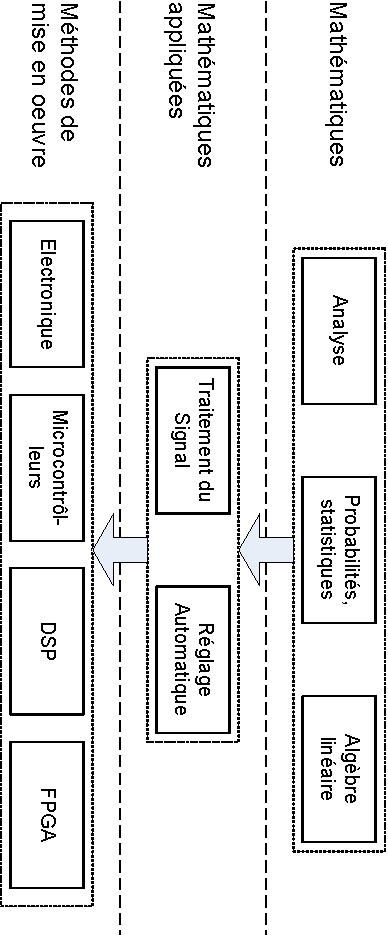
\includegraphics[angle=90, width=14cm]{./Chap01/Figures/Branches.pdf}
  \rule{35em}{0.5pt}
  \caption[Situation MUI]{Situation du cours MUI dans le cursus de l'ing�nieur}
  \label{fig:Branches}
\end{figure}


\section{D�finitions: processeur, microprocesseur, microcontr�leur et syst�me-on-chip}

Un processeur est un syst�me qui permet l'ex�cution d'op�rations �l�mentaires tel que des op�rations arithm�tiques (additions, soustractions, multiplication et division), des op�rations logiques (OR, AND, XOR), des tests (�gale �, plus petit que, etc.) et des d�placements de donn�es.

Le microprocesseur est un syst�me micro-�lectronique, aussi appel� circuit int�gr� ou plus commun�ment "chip" ou "puce", permettant l'ex�cution d'op�rations �l�mentaires. Contrairement au processeur qui est un concept, le microprocesseur est un composant que l'on place sur un circuit imprim�.

Un microcontr�leur est un syst�me micro-�lectronique contenant un microprocesseur et des p�riph�riques. Les p�riph�riques essentiels sont les minuteries, les interfaces de communication s�rie et les m�moires (donn�es et instructions).

Le syst�me-on-chip est en ensemble, diff�rent du microcontr�leur, qui inclut tout les composants �lectroniques d'un ordinateur � part les m�moires. Il se pr�sente sous la forme d'un circuit int�gr�. La m�moire de donn�es peut dans certain cas �tre assembl�e en dessus du chip pour r�duire la taille du syst�me.

\section{Analogie d'un processeur}

Pour expliquer le fonctionnement d'un processeur on peut en faire l'analogie avec un piano m�canique.

\section{�l�ments de syst�mes logiques}

Pour pouvoir configurer un microcontr�leur de mani�re efficace, nous avons besoins de quelques �l�ments de syst�mes logiques.

\begin{table}[!htbp]
\begin{center}
%\begin{tabular}{|p{.5cm}|c||c|c|c|c|c|c|c|c|c|c|c|c|c|c|c|c|}
\begin{tabular}{|c|c|*{16}{|c}|}
\hline 
\multicolumn{2}{|c|}{Variables} & \multicolumn{16}{|c|}{Fonctions}\\
\hline 
A & B & F0 & F1 & F2 & F3 & F4 & F5 & F6 & F7 & F8 & F9 & F10 & F11 & F12 & F13 & F14 & F15\\
\hline  
\hline 
0 & 0 & 0 & 0 & 0 & 0 & 0 & 0 & 0 & 0 & 1 & 1 & 1 & 1 & 1 & 1 & 1 & 1\\
\hline 
0 & 1 & 0 & 0 & 0 & 0 & 1 & 1 & 1 & 1 & 0 & 0 & 0 & 0 & 1 & 1 & 1 & 1\\
\hline
1 & 0 & 0 & 0 & 1 & 1 & 0 & 0 & 1 & 1 & 0 & 0 & 1 & 1 & 0 & 0 & 1 & 1\\
\hline
1 & 1 & 0 & 1 & 0 & 1 & 0 & 1 & 0 & 1 & 0 & 1 & 0 & 1 & 0 & 1 & 0 & 1\\
\hline
\end{tabular}
$\begin{array}{rclrclcl} \\
F0&=& 0 & \quad F15&=&\overline{F0}&=&1 \\ 
F1&=&A\cdot B & \quad F14&=&\overline{F1}&=&\overline{A \cdot B} \\
F2&=&A \cdot \overline{B} & \quad F13&=&\overline{F2}&=&\overline{A}+B  \\
F3&=&A & \quad F12&=&\overline{F3}&=&\overline{A}  \\
F4&=&\overline{A} \cdot B & \quad F11&=&\overline{F4}&=&A + \overline{B} \\
F5&=&B & \quad F10&=&\overline{F5}&=&\overline{B} \\
F6&=&A \oplus B & \quad F9&=&\overline{F6}&=&\overline{A \oplus B} \\
F7&=&A+B & \quad F8&=&\overline{F7}&=&\overline{A+B} 
\end{array}$
\end{center}

\caption{R�sultats possibles de fonctions � deux variables \label{variable_logiques}}
\end{table}

{\fontfamily{pcr}\selectfont Th�orie et traitement des signaux}

{\fontfamily{ppl}\selectfont Th�orie et traitement des signaux}

{\fontfamily{cmr}\selectfont Th�orie et traitement des signaux}

{\fontfamily{phv}\selectfont Th�orie et traitement des signaux}

\begin{center}
{\fontfamily{phv}\selectfont  Table Helvetica ou Arial\\
\begin{tabular}{|c|c|*{16}{|c}|}
\hline 
\multicolumn{2}{|c|}{Variables} & \multicolumn{16}{|c|}{Fonctions}\\
\hline 
A & B & F0 & F1 & F2 & F3 & F4 & F5 & F6 & F7 & F8 & F9 & F10 & F11 & F12 & F13 & F14 & F15\\
\hline  
\hline 
0 & 0 & 0 & 0 & 0 & 0 & 0 & 0 & 0 & 0 & 1 & 1 & 1 & 1 & 1 & 1 & 1 & 1\\
\hline 
0 & 1 & 0 & 0 & 0 & 0 & 1 & 1 & 1 & 1 & 0 & 0 & 0 & 0 & 1 & 1 & 1 & 1\\
\hline
1 & 0 & 0 & 0 & 1 & 1 & 0 & 0 & 1 & 1 & 0 & 0 & 1 & 1 & 0 & 0 & 1 & 1\\
\hline
1 & 1 & 0 & 1 & 0 & 1 & 0 & 1 & 0 & 1 & 0 & 1 & 0 & 1 & 0 & 1 & 0 & 1\\
\hline
\end{tabular}
}
\end{center}

\begin{thebibliography}{1}

\bibitem[1]{decoulon}Fr�d�ric de Coulon, \emph{Th�orie et traitement des signaux}, Presses polytechniques romandes, 1990

\bibitem[2]{proakis}John G. Proakis, Dimitris G. Manolakis: \emph{Digital Signal Processing}, Pearson Prentice Hall, 2007

\end{thebibliography}
 
%
%\pagenumbering{arabic} \setcounter{page}{1}
\chapter{\textsc{Num�ration et arithm�tique des ordinateurs}}

bla bla bla


\section{Repr�sentation des nombres}

\subsection{Entiers}

\subsection{Virgule flottante}

\subsection{Virgule fixe}


\section{Op�rateurs}

\subsection{Addition}

\subsection{Soustraction}

\subsection{Multiplication}


\section{Exercices}


\paragraph{Ex 1}


 

%\pagenumbering{arabic} \setcounter{page}{1}
\chapter{I\textsc{interfaces s�ries}}

Bla bla bla


\section{Notion de pile protocolaire}


\subsection{Mod�le OSI}






    %%  

%\input{./Chap04/Chapter04.tex}    % 
 
%\input{./Chap05/Chapter05.tex}    % 

\appendix


\chapter{\textsc{Analyse des syst�mes lin�aires}}

Bla bla bla


\section{La transformation de Laplace}


\subsection{Rappels math�matiques}


\paragraph{D�finition}

   %


\bigskip
\end{document}